%% Bookheader, Nov 8, 2020; July 18, 2022

\documentclass[11pt]{../Support/ourbook}
%% or for landscape, comment out line above and use this one:
%%\documentclass[landscape,11pt]{ourbook}

%% This will keep space from stretching around display math:

\makeatletter
\renewcommand\normalsize{%
   \@setfontsize\normalsize\@xipt{13.6}%
   \abovedisplayskip 11\p@  \@minus6\p@
   \abovedisplayshortskip \z@ 
   \belowdisplayshortskip 6.5\p@ \@minus3\p@
   \belowdisplayskip \abovedisplayskip
   \let\@listi\@listI}
\makeatother
\normalsize


\begin{document}

\tableofcontents
\graphicspath{{../../Chapters/vectors_matrices/en_US}}
\chapter{Vectors and Matrices}

The last chapter provided an overview of linear algebra, using several image
examples. In this chapter, we will focus primarily on vector-matrix
multiplications. First, we will show how matrices can be used to represent a
set of linear equations. Then, we will provide you with a general definition
of vector-matrix multiplication, followed by a few examples. You will have an
opportunity to solve a problem manually, then by using Python. In this
chapter, we will use two-dimensional matrices for simplicity, but a matrix can
have any number of dimensions.
\index{matrices}
\section{Matrices}
We've been looking at vectors. We've seen them in physics as a straight line comprised of $x$ and $y$ components, or represented as a column of
numbers. For example, while we may write $\mathbf{v} = \left[ 1, 2, 3 \right]$
in line, the vector is really:
$$\mathbf{v} = \begin{bmatrix}
1\\
2\\
3
\end{bmatrix}$$

A matrix can be made of many columns, like the $3 \times 2$ matrix shown below:
$$\begin{bmatrix}
1 & 1 & 1\\
2 & 4 & 8\\
3 & 9 & 27
\end{bmatrix}$$
\index{matrices!vector in form of}
We describe the size and shape of matrices by saying \textit{an }$m \times
n$\textit{ matrix}, where $m$ is the number of \emph{rows} and $n$ is the number of
\emph{columns}. A vector is simply a one-column matrix. For example, the vectors
\textbf{v} above is $3 \times 1$. Matrices aren't restricted to 2 dimensions:
a matrix can be 3, 4, or any number of dimensions. For example, a $3 \times 2
\times 4$ matrix would be made of 4 stacked $3 \times 2$ matrices.

\begin{Exercise}[title = {Matrix Dimensions 1}, label = mat_dim1]
Write the dimensions of the following matrices:
\begin{enumerate}
\item $\begin{bmatrix}
-3 & 0 & 4 & -2 & -4\\
-1 & 5 & 3 & 4 & -2\\
-3 & 2 & 3 & -5 & 1
\end{bmatrix}$
\item $\begin{bmatrix}
-3 & 1
\end{bmatrix}$
\item $\begin{bmatrix}
-3 & 2 & -3\\
4 & 0 & -3\\
-5 & -4 & 1\\
0 & -2 & 2\\
\end{bmatrix}$
\end{enumerate}
\end{Exercise}

\begin{Answer}[ref = mat_dim1]
\begin{enumerate}
\item $3 \times 5$
\item $1 \times 2$
\item $4 \times 3$
\end{enumerate}
\end{Answer}

\begin{Exercise}[title = {Matrix Dimensions 2}, label = mat_dim2]
Create a matrix with the indicated dimensions.
\begin{enumerate}
\item $1 \times 3$
\item $2 \times 4$
\item $4 \times 3$
\end{enumerate}
\end{Exercise}

\begin{Answer}[ref = mat_dim2]
\begin{enumerate}
\item The matrix should have 1 row and 3 columns. For example,
$$\begin{bmatrix}
1 & 2 & 3
\end{bmatrix}$$
\item The matrix should have 2 rows and 4 columns. For example,
$$\begin{bmatrix}
1 & 2 & 3 & 4\\
5 & 6 & 7 & 8
\end{bmatrix}$$
\item The matrix should have 4 rows and 3 columns. For example,
$$\begin{bmatrix}
1 & 2 & 3\\
4 & 5 & 6\\
7& 8 & 9\\
10 & 11 & 12
\end{bmatrix}$$
\end{enumerate}
\end{Answer}

\subsection{Zero Matrices}
Recall that we can represent a generic zero vector as \textbf{0} or \vec{0} (you may see both), which
indicates a vector of any number of dimensions filled with zeros. Just like
vectors, there are \textit{zero matrices}\index{zero matrix}, which can be any number of dimensions, all filled with zeros. 
In two dimensions, zero matrices are denoted as $\mathbf{\mathit{0}}_{m \times n}$, where the
subscript is the dimension of the matrix. The subscript can be expanded to
denote any number of dimensions.

\section{Operations of Matrices}
\subsection{Adding and Subtracting Matrices}
Matrices that are the same dimension can be added and subtracted. Just like
vectors, to add matrices you add the elements in the same position:
$$\begin{bmatrix}
-2 & -1\\
2 & 4
\end{bmatrix}
+ \begin{bmatrix}
5 & 2\\
-1 & -4
\end{bmatrix}
= \begin{bmatrix}
-2 + 5 & -1 + 2\\
2 + -1 & 4 + -4
\end{bmatrix} =
\begin{bmatrix}
3 & 1\\
1 & 0
\end{bmatrix}$$

And to subtract matrices, you subtract the elements in the same position:
$$\begin{bmatrix}
-2 & -1\\
2 & 4
\end{bmatrix}
- \begin{bmatrix}
5 & 2\\
-1 & -4
\end{bmatrix}
= \begin{bmatrix}
-2 - 5 & -1 - 2\\
2 - (-1) & 4 - (-4)
\end{bmatrix} =
\begin{bmatrix}
-7 & -3\\
3 & 8
\end{bmatrix}$$

Formally, for 2-dimensional matrices, we can say that:
\begin{mdframed}[style = important, frametitle={Adding and Subtracting Matrics}]
For two $m \times n$ matrices, the sum of the matrices is the matrix of the
sums of the elements in analogous positions:
$$\begin{bmatrix}
x_{11} & x_{12} & x_{13} & \cdots & x_{1n}\\
x_{21} & x_{22} & x_{23} & \cdots & \vdots\\
\vdots & \vdots & \vdots & \cdots & \vdots\\
x_{m1} & x_{m2} & x_{m3} & \cdots & x_{mn}
\end{bmatrix}
+ \begin{bmatrix}
y_{11} & y_{12} & y_{13} & \cdots & y_{1n}\\
y_{21} & y_{22} & y_{23} & \cdots & \vdots\\
\vdots & \vdots & \vdots & \cdots & \vdots\\
y_{m1} & y_{m2} & y_{m3} & \cdots & y_{mn}
\end{bmatrix} = $$
$$\begin{bmatrix}
x_{11} + y_{11} & x_{12} + y_{12} & x_{13} + y_{13} & \cdots & x_{1n} + y_{1n}\\
x_{21} + y_{21} & x_{22} + y_{22} & x_{23} + y_{23} & \cdots & \vdots\\
\vdots & \vdots & \vdots & \cdots & \vdots\\
x_{m1} + y_{m1} & x_{m2} + y_{m2} & x_{m3} + y_{m3} & \cdots & x_{mn} + y_{mn}
\end{bmatrix}$$

To subtract matrices, simply add the negative of the second matrix (that is,
\textbf{\textit{A}} - \textbf{\textit{B}} = \textbf{\textit{A}} + -\textbf{
\textit{B}}). Additionally, matrix addition is commutative (\textbf{\textit{A}}
+ \textbf{\textit{B}} = \textbf{\textit{B}} + \textbf{\textit{A}}).

Matrices of different dimensions cannot be added or subtracted. 
\end{mdframed}

\begin{Exercise}[title = {Adding and Subtracting Matrices}, label = add_mat]
Find \textbf{\textit{A}} + \textbf{\textit{B}}, \textbf{\textit{A}} -
\textbf{\textit{B}}, and \textbf{\textit{B}} - \textbf{\textit{A}}.
\begin{enumerate}
\item $\textbf{\textit{A}} = \begin{bmatrix}
0 & 4 & 0 & 5
\end{bmatrix}$ and $\textbf{\textit{B}} = \begin{bmatrix}
-2 & 3 & -2 & 5
\end{bmatrix}$
\item $\textbf{\textit{A}} = \begin{bmatrix}
4 & -4 & -2\\
1 & -3 & 5\\
-5 & 3 & 0
\end{bmatrix}$ and $\textbf{\textit{B}} = \begin{bmatrix}
5 & 0 & -1\\
-5 & -3 & -2\\
-5 & 3 & -4
\end{bmatrix}$.
\item $\textbf{\textit{A}} = \begin{bmatrix}
-2 & -1 & -5 & -1\\
5 & -4 & 4 & 3
\end{bmatrix}$ and $\textbf{\textit{B}} = \begin{bmatrix}
-5 & -2 & 3 & -5\\
0 & 5 & -4 & -3
\end{bmatrix}$.
\end{enumerate}
\end{Exercise}

\begin{Answer}[ref = add_mat]
\begin{enumerate}
\item \textbf{\textit{A}} + \textbf{\textit{B}} $= \begin{bmatrix}
-2 & 7 & -2 & 10
\end{bmatrix}$. $\textbf{\textit{A}} - \textbf{\textit{B}} = \begin{bmatrix}
2 & 1 & 2 & 0
\end{bmatrix}$. $\textbf{\textit{B}} - \textbf{\textit{A}} = \begin{bmatrix}
-2 & -1 & -2 & 0
\end{bmatrix}$
\item $\textbf{\textit{A}} + \textbf{\textit{B}} = \begin{bmatrix}
9 & -4 & -3\\
-4 & -6 & 3\\
-10 & 6 & -4
\end{bmatrix}$. $\textbf{\textit{A}} - \textbf{\textit{B}} = \begin{bmatrix}
-1 & -4 & -1\\
6 & 0 & 7\\
0 & 0 & 4
\end{bmatrix}$. $\textbf{\textit{B}} - \textbf{\textit{A}} = \begin{bmatrix}
1 & 4 & 1\\
-6 & 0 & -7\\
0 & 0 & -4
\end{bmatrix}$.
\item $\textbf{\textit{A}} + \textbf{\textit{B}} = \begin{bmatrix}
-7 & -3 & -2 & -6\\
5 & 1 & 0 & 0
\end{bmatrix}$. $\textbf{\textit{A}} - \textbf{\textit{B}} = \begin{bmatrix}
3 & 1 & -8 & 4\\
5 & -9 & 8 & 6
\end{bmatrix}$. $\textbf{\textit{B}} - \textbf{\textit{A}} = \begin{bmatrix}
-3 & -1 & 8 & -4\\
-5 & 9 & -8 & -6
\end{bmatrix}$.
\end{enumerate}
\end{Answer}

\subsection{Multiplying Matrices}
Surprisingly (it may be to you), matrix multiplication has dimension limits.
We cannot multiply any two matrices: the first matrix must have the same
number of columns as the second has number of rows. Let's examine the origin
of the dimension limits on matrix multiplication. We begin with a review of
the vector dot product.

Recall that in order to find the dot product of two vectors, they must be the
same length (that is, the same number of dimensions). The result is always a
scalar: one number. You can review finding the dot product of vectors and
practice the dimension limits on the vector dot product in the next exercise.

\begin{Exercise}[title = {Vector Dot Product Review}, label = vect_dot]
Find all possible pairs of vectors that can be used to find a dot product,
then find the dot products.
\begin{enumerate}
\item $\mathbf{a} = \begin{bmatrix}
1\\
2
\end{bmatrix}$
\item $\mathbf{b} = \begin{bmatrix}
-3\\
3\\
5\\
-5
\end{bmatrix}$
\item $\mathbf{c} = \begin{bmatrix}
1\\
2\\
-1
\end{bmatrix}$
\item $\mathbf{d} = \begin{bmatrix}
-5\\
-1
\end{bmatrix}$
\item $\mathbf{e} = \begin{bmatrix}
1\\
-5\\
3\\
1
\end{bmatrix}$
\item $\mathbf{f} = \begin{bmatrix}
4\\
1\\
-3
\end{bmatrix}$
\end{enumerate}
\end{Exercise}

\begin{Answer}[ref = vect_dot]
It is possible to compute $\mathbf{a} \cdot \mathbf{d}$, $\mathbf{b} \cdot
\mathbf{e}$, and $\mathbf{c} \cdot \mathbf{f}$:
\begin{enumerate}
    \item $\mathbf{a} \cdot \mathbf{d} = 1(-5) + 2(-1) = -5 + (-2) = -7$
    \item $\mathbf{b} \cdot \mathbf{e} = -3(1) + 3(-5) + 5(3) + -5(1) = -3 +
    (-15) + 15 - 5 = -8$
    \item $\mathbf{c} \cdot \mathbf{f} = 1(4) + 2(1) + -1(-3) = 4 + 2 + 3 = 9$
\end{enumerate}
\end{Answer}

To multiply two matrices, it is helpful to think of the rows of the first
matrix and the columns of the second matrix as vectors. Let's see how this
shakes out for two $2 \times 2$ matrices:

\begin{figure}
    \centering
    \begin{tikzpicture}
        \node[] at (0,0) {$\begin{bmatrix}
            5 & 4\\
            -5 & 1
        \end{bmatrix} \cdot \begin{bmatrix}
            -1 & -2\\
            -5 & -4
        \end{bmatrix} = \begin{bmatrix}
             & & & & & & & \\
             & & & & & & &
        \end{bmatrix}$};
        \node[] at (-2.75, -1) {\textbf{\textit{A}}};
        \node[] at (-2, -1) {$\cdot$};
        \node[] at (-1, -1) {\textbf{\textit{B}}};
        \node[text = red] at (-3.8, 0.25) {$\mathbf{a}_1 \to$};
        \node[text = red] at (-3.8, -0.25) {$\mathbf{a}_2 \to$};
        \node[text = blue] at (-1.3, 0.7) {$\downarrow$};
        \node[text = blue] at (-1.3, 1) {$\mathbf{b}_1$};
        \node[text = blue] at (-0.55, 0.7) {$\downarrow$};
        \node[text = blue] at (-0.55, 1) {$\mathbf{b}_2$};
        \node[text = red] at (0.95, 0.15) {$\mathbf{a}_1$};
        \node[] at (1.2, 0.15) {$\cdot$};
        \node[text = blue] at (1.5, 0.15) {$\mathbf{b}_1$};
        \node[text = red] at (0.95, -0.25) {$\mathbf{a}_2$};
        \node[] at (1.2, -0.25) {$\cdot$};
        \node[text = blue] at (1.5, -0.25) {$\mathbf{b}_1$};
        \node[text = red] at (2.15, 0.15) {$\mathbf{a}_1$};
        \node[] at (2.4, 0.15) {$\cdot$};
        \node[text = blue] at (2.7, 0.15) {$\mathbf{b}_2$};
        \node[text = red] at (2.15, -0.25) {$\mathbf{a}_2$};
        \node[] at (2.4, -0.25) {$\cdot$};
        \node[text = blue] at (2.7, -0.25) {$\mathbf{b}_2$};
    \end{tikzpicture}
    \caption{Each entry in \textbf{\textit{C}}, $c_{ij}$, is the dot product
    of the $i^{th}$ row of \textbf{\textit{A}}, $a_i$, and the $j^{th}$ column
    of \textbf{\textit{B}}, $b_j$.}
    \label{fig:mat_mult}
\end{figure}

 Let's look at this more concretely. For two-dimensional matrices, it can be
 helpful to move your left index finger across the row and right index finger
 down the column, as shown in figure \ref{fig:fingers}.

 \begin{figure}[htbp]
    \centering
    \begin{tikzpicture}
        \node[] at (0,3) {$\begin{bmatrix}
            5 & 4\\
            -5 & 1
        \end{bmatrix} \cdot \begin{bmatrix}
            -1 & -2\\
            -5 & -4
        \end{bmatrix} = \begin{bmatrix}
             & & & & & & & \\
             & & & & & & &
        \end{bmatrix}$};
        \draw[thick, -latex, red] (-3, 3.25) -- (-2, 3.25);
        \draw[thick, -latex, blue] (-1.25, 3.4) -- (-1.25, 2.6);
        \node[font = \tiny] at (1.25, 3.25) {
        \textcolor{red}{5}$\times$\textcolor{blue}{-1}$+$\textcolor{red}{4}$\times$\textcolor{blue}{-4}};

        \node[] at (0,2) {$\begin{bmatrix}
            5 & 4\\
            -5 & 1
        \end{bmatrix} \cdot \begin{bmatrix}
            -1 & -2\\
            -5 & -4
        \end{bmatrix} = \begin{bmatrix}
             & & & & & & & \\
             & & & & & & &
        \end{bmatrix}$};
        \draw[thick, -latex, red] (-3, 2.25) -- (-2, 2.25);
        \draw[thick, -latex, blue] (-.35, 2.4) -- (-.35, 1.6);
        \node[font = \normalsize] at (1.25, 2.25) {-21};
        \node[font = \tiny] at (2.25, 2.25) {
        \textcolor{red}{5}$\times$\textcolor{blue}{-2}$+$\textcolor{red}{4}$\times$\textcolor{blue}{-4}};

        \node[] at (0, 1) {$\begin{bmatrix}
            5 & 4\\
            -5 & 1
        \end{bmatrix} \cdot \begin{bmatrix}
            -1 & -2\\
            -5 & -4
        \end{bmatrix} = \begin{bmatrix}
             & & & & & & & \\
             & & & & & & &
        \end{bmatrix}$};
        \draw[thick, -latex, red] (-3, 0.75) -- (-2, 0.75);
        \draw[thick, -latex, blue] (-1.25, 1.4) -- (-1.25, 0.6);
        \node[font = \normalsize] at (1.25, 1.25) {-21};
        \node[font = \normalsize] at (2.25, 1.25) {-26};
        \node[font = \tiny] at (1.25, 0.8) {
        \textcolor{red}{-5}$\times$\textcolor{blue}{-1}$+$\textcolor{red}{1}$\times$\textcolor{blue}{-5}};

        \node[] at (0,0) {$\begin{bmatrix}
            5 & 4\\
            -5 & 1
        \end{bmatrix} \cdot \begin{bmatrix}
            -1 & -2\\
            -5 & -4
        \end{bmatrix} = \begin{bmatrix}
             & & & & & & & \\
             & & & & & & &
        \end{bmatrix}$};
        \draw[thick, -latex, red] (-3, -0.25) -- (-2, -0.25);
        \draw[thick, -latex, blue] (-.35, 0.4) -- (-.35, -0.4);
        \node[font = \normalsize] at (1.25, 0.25) {-21};
        \node[font = \normalsize] at (2.25, 0.25) {-26};
        \node[font = \normalsize] at (1.25, -0.25) {0};
        \node[font = \tiny] at (2.25, -0.25) {
        \textcolor{red}{-5}$\times$\textcolor{blue}{-2}$+$\textcolor{red}{1}$\times$\textcolor{blue}{-4}};
        \node[] at (0,-1) {$\begin{bmatrix}
            5 & 4\\
            -5 & 1
        \end{bmatrix} \cdot \begin{bmatrix}
            -1 & -2\\
            -5 & -4
        \end{bmatrix} = \begin{bmatrix}
             & & & & & & & \\
             & & & & & & &
        \end{bmatrix}$};
        \node[font = \normalsize] at (1.25, -0.75) {-21};
        \node[font = \normalsize] at (2.25, -0.75) {-26};
        \node[font = \normalsize] at (1.25, -1.25) {0};
        \node[font = \normalsize] at (2.25, -1.25) {6};
    \end{tikzpicture}
    \caption{You can use your fingers to trace across matrix \textbf{\textit{A}}
    and down matrix \textbf{\textit{B}} to find $\textbf{\textit{A}} \cdot
    \textbf{\textit{B}}$.}
    \label{fig:fingers}
\end{figure}

Since each entry in the product matrix is the dot product between a row of the
first matrix and a column of the second matrix, the first matrix must have the
same number of elements in each row as the second has in each column. Another
way to say this is that the number of columns of the first matrix must match
the number of rows in the second matrix.

\begin{mdframed}[style = important, frametitle = {Matrix Multiplication}]
For two-dimensional matrices, the inner dimensions must match in order to
carry out matrix multiplication. That is, if we want to find \textbf{\textit{
A}}$\cdot$\textbf{\textit{B}}, and \textbf{\textit{A}} has dimensions $m
\times n$, then \textbf{\textit{B}} must have dimensions $n \times p$, where
$m$, $n$, and $p$ are integers. The resulting matrix will have dimensions $m
\times p$ ($m$ and $p$ may be equal or unequal).
\end{mdframed}

\begin{Exercise}[title = {Multiplying Matrices 1}, label = mult_mat1]
Multiply the matrices.
\begin{enumerate}
\item $\begin{bmatrix}
-5 & -2 & 2 & 1
\end{bmatrix} \cdot \begin{bmatrix}
-3 & -1 & -5\\
3 & 0 & 3\\
4 & -1 & -4\\
-1 & -4 & 2
\end{bmatrix}$
\item $\begin{bmatrix}
1\\
5\\
-5\\
4\\
1
\end{bmatrix} \cdot \begin{bmatrix}
0 & 5 & 1
\end{bmatrix}$
\item $\begin{bmatrix}
-1 & 4 & -4\\
5 & -3 & 5\\
-1 & -4 & 4\\
-4 & 1 & 4
\end{bmatrix} \cdot \begin{bmatrix}
-3 & 5 & 1\\
-3 & 0 & -3\\
0 & 3 & 0
\end{bmatrix}$
\end{enumerate}
\end{Exercise}

\begin{Answer}[ref = mult_mat1]
\begin{enumerate}
    \item $\begin{bmatrix}
        -2 & -1 & 5
    \end{bmatrix}$
    \item $\begin{bmatrix}
        0 & 5 & 1\\
        0 & 25 & 5\\
        0 & -25 & -5\\
        0 & 20 & 4\\
        0 & 5 & 1
    \end{bmatrix}$
    \item $\begin{bmatrix}
        -9 & -17 & 11\\
        -6 & 40 & -4\\
        15 & 7 & -13\\
        9 & -8 & -1
    \end{bmatrix}$
\end{enumerate}
\end{Answer}

\begin{Exercise}[title = {Multiplying Matrices 2}, label = mult_mat2]
Find $\mathbf{\mathit{A}} \cdot \mathbf{\mathit{B}}$ and $\mathbf{\mathit{B}} \cdot \mathbf{\mathit{A}}$.
\begin{enumerate}
\item $\mathbf{\mathit{A}} = \begin{bmatrix}
-2\\
2\\
1\\
-2
\end{bmatrix}$ and $\mathbf{\mathit{B}} = \begin{bmatrix}
-4 & 3 & -5 & -2
\end{bmatrix}$
\item $\mathbf{\mathit{A}} = \begin{bmatrix}
-4 & -2\\
2 & 5\\
-3 & -4\\
\end{bmatrix}$ and $\mathbf{\mathit{B}} = \begin{bmatrix}
0 & -2 & -4\\
1 & -4 & 0
\end{bmatrix}$
\item $\mathbf{\mathit{A}} = \begin{bmatrix}
2 & 0 & 1 & 4\\
-4 & 0 & -5 & -1
\end{bmatrix}$ and $\mathbf{\mathit{B}} = \begin{bmatrix}
0 & -3\\
-4 & -1\\
-2 & 3\\
-5 & 1
\end{bmatrix}$
\end{enumerate}
\end{Exercise}

\begin{Answer}[ref = mult_mat2]
\begin{enumerate}
\item $\mathbf{\mathit{A}} \cdot \mathbf{\mathit{B}} = \begin{bmatrix}
8 & -6 & 10 & 4\\
-8 & 6 & -10 & -4\\
-4 & 3 & -5 & -2\\
8 & -6 + 1- & 4
\end{bmatrix}$ and $\mathbf{\mathit{B}} \cdot \mathbf{\mathit{A}} =
\begin{bmatrix}
13
\end{bmatrix}$
\item $\mathbf{\mathit{A}} \cdot \mathbf{\mathit{B}} = \begin{bmatrix}
-2 & 16 & 16\\
5 & -24 & -8\\
-4 & 22 & 12
\end{bmatrix}$ and $\mathbf{\mathit{B}} \cdot \mathbf{\mathit{A}} =
\begin{bmatrix}
8 & 6\\
-12 & -22
\end{bmatrix}$
\item $\mathbf{\mathit{A}} \cdot \mathbf{\mathit{B}} = \begin{bmatrix}
-22 & 1\\
15 & -4
\end{bmatrix}$ and $\mathbf{\mathit{B}} \cdot \mathbf{\mathit{A}} =
\begin{bmatrix}
12 & 0 & 15 & 3\\
-4 & 0 & 1 & -15\\
-16 & - & -17 & -11\\
-14 & 0 & -10 & -21
\end{bmatrix}$
\end{enumerate}
\end{Answer}

What have you noticed about the results of $\mathbf{\mathit{A}} \cdot
\mathbf{\mathit{B}}$ as compared to $\mathbf{\mathit{B}} \cdot \mathbf{
\mathit{A}}$? You should have noticed that the product matrices are
\textit{different dimensions}. This leads us to the next unusual property of
matrix multiplication: it is \textit{non-commutative}. That is, the \textit{
order} in which you multiply matrices affects the result. This is very
different from scalar values!

As you saw in the second matrix multiplication exercise, \textbf{\textit{A}}
is a $2 \times 4$ matrix and \textbf{\textit{B}} is a $4 \times 2$ matrix,
then \textbf{\textit{A}}\textbf{\textit{B}} is a $2 \times 2$ matrix, while
\textbf{\textit{B}}\textbf{\textit{A}} is a $4 \times 4$ matrix. It is obvious,
then, that $\mathbf{\mathit{A}} \cdot \mathbf{\mathit{B}} \neq \mathbf{\mathit{
B}} \cdot \mathbf{\mathit{A}}$. What if \textbf{\textit{A}} and \textbf{\textit{
B}} are square matrices?

\textbf{Example}: Find $\mathbf{\mathit{A}} \cdot \mathbf{\mathit{B}}$ and
$\mathbf{\mathit{B}} \cdot \mathbf{\mathit{A}}$ if $\mathbf{\mathit{A}} =
\begin{bmatrix}
-3 & 5\\
-1 & 0
\end{bmatrix}$ and $\mathbf{\mathit{B}} = \begin{bmatrix}
-1 & 1\\
4 & -3
\end{bmatrix}$.

\textbf{Solution}: $$\mathbf{\mathit{A}} \cdot \mathbf{\mathit{B}} =
\begin{bmatrix}
-3 & 5\\
-1 & 0
\end{bmatrix} \cdot \begin{bmatrix}
-1 & 1\\
4 & -3
\end{bmatrix} = \begin{bmatrix}
-3(-1) + 5(4) & -3(1) + 5(-3)\\
-1(-1) + 0(4) & -1(1) + 0(-3)
\end{bmatrix} = \begin{bmatrix}
23 & -18\\
1 & -1
\end{bmatrix}$$

$$\mathbf{\mathit{B}} \cdot \mathbf{\mathit{A}} = \begin{bmatrix}
-1 & 1\\
4 & -3
\end{bmatrix} \cdot \begin{bmatrix}
-3 & 5\\
-1 & 0
\end{bmatrix} = \begin{bmatrix}
-1(-3) + 1(-1) & -1(5) + 1(0)\\
4(-3) + -3(-1) & 4(5) + -3(0)
\end{bmatrix} = \begin{bmatrix}
2 & -5\\
-9 & 20
\end{bmatrix}$$

As you can see, even if \textbf{\textit{A}} and \textbf{\textit{B}} are square,
matrix multiplication is still not commutative.

\begin{mdframed}[style = important, frametitle = {Non-Commutation of Matrix Multiplication}]
For two matrices \textbf{\textit{A}} and \textbf{\textit{B}}, where neither is
an identity matrix or a zero matrix:
$$\mathbf{\mathit{A}} \cdot \mathbf{\mathit{B}} \neq \mathbf{\mathit{B}}
\cdot \mathbf{\mathit{A}}$$
\end{mdframed}

\subsubsection{Properties of the Zero Matrix}
Just like the number 0, the zero matrix, \textbf{\textit{O}} has unique
mathematical properties:
\begin{mdframed}[style = important, frametitle = {Properties of the Zero Matrix}]
For a matrix, \textbf{\textit{A}}, and a zero matrix, \textbf{\textit{O}}
\begin{enumerate}
\item $\mathbf{\mathit{A}} + \mathbf{\mathit{O}} = \mathbf{\mathit{A}}$
\item $\mathbf{\mathit{A}} + \mathbf{\mathit{-A}} = \mathbf{\mathit{O}}$
\item $0 \cdot \mathbf{\mathit{A}} = \mathbf{\mathit{O}}$
\end{enumerate}
\end{mdframed}

\subsubsection{The Identity Matrix}
There is another special matrix, called the \textit{identity matrix}\index{
identity matrix}, usually denoted with \textbf{\textit{I}}. An identity matrix
is all zeroes except for a diagonal line of ones. A $3 \times 3$ identity
matrix is shown below:

$$\begin{bmatrix}
1 & 0 & 0\\
0 & 1 & 0\\
0 & 0 & 1
\end{bmatrix}$$

All identity matrices are square (that is, they have the same number of rows
as they do columns). The identity matrix has the special property that
whenever a vector or matrix is multiplied by \textbf{\textit{I}}, it doesn't
change. Let's look at some examples:

\textbf{Example}: If $\mathbf{x} = \begin{bmatrix}
2\\
-3
\end{bmatrix}$, what is $\mathbf{\mathit{I}}\mathbf{x}$? (Take \textbf{\textit{
I}} to be a $2 \times 2$ identity matrix.)

\textbf{Solution}: $$\mathbf{\mathit{I}} \mathbf{x} = \begin{bmatrix}
1 & 0 \\
0 & 1
\end{bmatrix} \cdot \begin{bmatrix}
2 \\
-3
\end{bmatrix} = \begin{bmatrix}
1 \cdot (2) + 0 \cdot (-3)\\
0 \cdot (2) + 1 \cdot (-3)
\end{bmatrix} = \begin{bmatrix}
2\\
-3
\end{bmatrix}$$

\textbf{Example}: If $\mathbf{\mathit{B}} = \begin{bmatrix}
-2 & 5\\
3 & -4
\end{bmatrix}$, what is $\mathbf{\mathit{I}} \cdot \mathbf{\mathit{B}}$?

\textbf{Solution}: $$\mathbf{\mathit{I}} \cdot \mathbf{\mathit{B}} =
\begin{bmatrix}
1 & 0 \\
0 & 1
\end{bmatrix} \cdot \begin{bmatrix}
-2 & 5\\
3 & -4
\end{bmatrix} = \begin{bmatrix}
1 \cdot (-2) + 0 \cdot (5) & 1 \cdot (5) + 0 \cdot (-4)\\
0 \cdot (-2) + 1 \cdot (5) & 0 \cdot (5) + 1 \cdot (-4)
\end{bmatrix} = \begin{bmatrix}
-2 & 5\\
3 & -4
\end{bmatrix}$$

\begin{mdframed}[style = important, frametitle = {Properties of the Identity Matrix}]
An $n \times n$ identity matrix, \textbf{\textit{I}}, does not change any
vectors or matrices it multiplies. That is:
\begin{enumerate}
\item $\mathbf{\mathit{I}} \cdot \mathbf{x} = \mathbf{x}$
\item $\mathbf{\mathit{I}} \cdot \mathbf{\mathit{B}} = \mathbf{\mathit{B}}$
\end{enumerate}
where \textbf{x} is an $n \times 1$ vector and \textbf{\textit{B}} is an $n
\times p$ matrix ($p$ may be, but is not necessarily, equal to $n$).
\end{mdframed}

\subsection{Can We Divide Matrices?}
Matrices cannot be divided. Suppose we have a matrix, \textbf{\textit{A}}, a vector \textbf{x}, and another vector \textbf{b} such that:

$$\textbf{\textit{A}} \cdot \textbf{x} = \textbf{b}$$

Now, if we know \textbf{\textit{A}} and \textbf{x}, it is easy to find \textbf{b}. What if, on the other hand, we know \textbf{\textit{A}} and \textbf{b} and want to find \textbf{x}? We might be tempted to do something like this:

$$\textbf{x} = \frac{\textbf{b}}{\textbf{\textit{A}}}$$

While this would be correct if \textbf{x}, \textbf{b}, and \textbf{\textit{A}} were scalars, but it is not for matrices. However, there is an analogy we can make. Instead of trying to divide by \textbf{\textit{A}}, we can multiply by its \textit{inverse}:

\begin{mdframed}[style = important, frametitle = {Inverse Matrices}]
Given a matrix \textbf{\textit{A}}, and vectors \textbf{b} and \textbf{x}, if

$$\textbf{\textit{A}} \cdot \textbf{x} = \textbf{b}$$

Then,

$$\textbf{x} = \textbf{\textit{A}}^{-1} \cdot \textbf{b}$$
\end{mdframed}

$\textbf{\textit{A}}^{-1}$ is called the \textit{inverse matrix}. We will explore inverse matrices and how to find them in the next chapter.

\graphicspath{{../../Chapters/linear_combinations/en_US}}
\chapter{Linear Combinations}

A linear combination of vectors is the addition of two or more scaled vectors. For example, given two vectors, ${v}_1, {v}_2$ and two scalars $a_1,a_2$, you'd write their linear combination as:

\[x
\mathbf{w} = a_1\mathbf{v}_1 + a_2\mathbf{v}_2
\]

The scalars can be any real number. The vectors can be of any dimension. 

Let's take a more generalized approach. Given vectors $\mathbf{v}_1,
\mathbf{v}_2, ..., \mathbf{v}_n \in \mathbb{R}^m$ and scalars $a_1,
a_2, ..., a_n \in \mathbb{R}$, a linear combination of these vectors
is any vector of the form\index{linear combinations}

\[
\mathbf{w} = a_1\mathbf{v}_1 + a_2\mathbf{v}_2 + ... + a_n\mathbf{v}_n
\]

Each scalar $a_i$ scales the corresponding vector $\mathbf{v}_i$, and
added together, the results are produce a new vector $\mathbf{w}$.

Let's look at an example that has 4 vectors and their scalars. 

$$a_1 = 1, v_1 = [9, 1, 2]$$
 $$a_2 = -1, v_2 = [8, -3, 4]$$
$$a_3 = 3, v_3 = [6, 0, 1]$$
$$a_4 = -4, v_4 = [3, 7, 2]$$

As a linear combination:

$$\mathbf{w} = 1*[9,1,2] + (-1)*[8, -3, 4]+ 3*[6,0,1] + (-4)*[3,7,2]$$

After multiplying each vector by its associated scalar.

$$\mathbf{w} = [9, 1, 2] + [-8, 3, -4] + [18, 0, 3] + [-12, -28, -8]$$

When combined:

$$\mathbf{w} = [7, -24, -7]$$


\begin{Exercise}[title={Linear Combination}, label=linearCombo]
Calculate the linear combination 
for vectors $v_1, v_2, v_3$ and
scalars $a_1, a_2,a_3$ where:   

$$a1 = 2, v1 =[2, 4, 8]$$
$$a2 = -2,v2 =[8, -6, 3]$$
$$a3 = 4,v3 =[7, 9, 2]$$

Make sure to show all your work. 
\end{Exercise}
\begin{Answer}[ref=linearCombo]
     \[
	\mathbf{w} = 2*[2,4,8] + (-2)*[8,-6,3] + 4*[7,9,2] 
	\]
  	\[
	\mathbf{w} = [4,8,16] + [-16,12,-6] + [28,36,8] 
	\]  
 	\[
	\mathbf{w} = [16, 56, 18]  
	\]   
\end{Answer}

\section{Weighted Averages of Vectors}
A weighted average of vectors is a specific type of linear combination
where the coefficients (or weights) $a_i$ are non-negative and sum to
1:\index{weighted averages}
\[
\sum_{i=1}^{n} a_i = 1, \quad a_i \geq 0
\]

A weighted average of vectors $\mathbf{v}_1, \mathbf{v}_2, ...,
\mathbf{v}_n$ is then defined as

\[
\mathbf{w} = a_1\mathbf{v}_1 + a_2\mathbf{v}_2 + ... + a_n\mathbf{v}_n
\]

In this case, each $a_i$ not only scales the corresponding vector
$\mathbf{v}_i$, but also represents the proportion of that vector in
the final average vector $\mathbf{w}$.

Weighted averages are useful when you want to attribute the contribution of one feature or item over another. For example, a teacher might figure a student's final grade using exam scores, class participation, and a final project. The exam scores might make up 65\% of the final grade, class participation 10\%, and a final project 25\%. Thus giving the formula for a grade as:

\[
\mathbf{Grade} = .65*ExamScores + .10*Participation + .25*FinalProject
\]

The teacher defines the weights, making sure they sum to 1.0. 

Let's look at an example where the weights don't sum to 1.0. A store that sells umbrellas might have to get the umbrella stock from three different manufacturers. The store owner buys 100 umbrellas at a cost of \$2.10 each, 50 umbrellas cost \$1.85 each, and 200 umbrellas cost \$2.00. 

\[
\mathbf{TotalCost} = 2.10*100 + 1.85*50 + 2.00*200 = 702.5
\]

To calculate the weighted average, divide the total cost by the number of items.

\[
\mathbf{WeightedAverage} = 702.5/350 = 2.01 
\]

\begin{Exercise}[title={Weighted Average}, label=weightedAverage]
A concert sells 300 tickets in the balcony at \$50 each, 100 tickets on the main floor at \$75 each, and 50 tickets in the section closest to the stage at \$150 each. What's the weighted average?
\end{Exercise}
\begin{Answer}[ref=weightedAverage]
\[\mathbf{TotalSales} = 50*300 + 75*100 + 150*50 = 30,000\]
\[\mathbf{NumberTickets} = 300 + 100 + 50 = 450\]
\[\mathbf{WeightedAverage} = 30,000/450 = 66.67\]
\end{Answer}

\section{Weighted Averages of Vectors in Python}
Create a file called \filename{linearCombos.py} and enter this code:

\begin{Verbatim}
// import the python module that supports matrices
import numpy as np

// an array for number of umbrellas by manufacturer
items = np.array([100, 50, 200])

// weights are the cost of item by manufacturer
weights = np.array([2.10, 1.85, 2.00])

// create an array for total cost for each manufacturer
costPerManufacturer=items * weights

// sum the individuals costs to get the total
totalCost = np.sum(costPerManufacturer)

// get number of items
numItems = np.sum(items) 

// you are ready to calculated the weighted average
weightedAverage = totalCost/numItems
print(weightedAverage)
\end{Verbatim}

When you run this code, you should get a weighted average of \$2.01 when rounded to the nearest cent.



\graphicspath{{../../Chapters/spans_independence/en_US}}
\chapter{Vector Spans and Independence}
Think back to a time when you played with blocks. If you had two blocks, you couldn't make many shapes out of them. With three, you had a few more options. With a dozen you were able to make many more shapes. In the world of blocks, a span would be all the things you could make with a given set of blocks. 

A vector span is similar, but in a mathematical sense. If I give you the coordinates for a vector and ask you to make everything you can from that vector using only the original vector, the result is the span. You can scale the vector, add it to itself, anything that is a linear combination of only that vector. As with the blocks, you'll find what you can make from one vector is limited. The span will be a line. But when you are given two or more vectors to "play" with, you will be able to create much more. The span will be larger than in the case of having only one vector. The size of the span (sometimes referred to as a subspace) will depend on whether the vectors are linearly independent or dependent. 

\section{Overview: Independence and Dependence}
A set of linearly independent vectors means that no vector is a combination of any other vector. Let's look at these three:
$$[1 0 0]$$
$$[0 1 0]$$
$$[0 0 1]$$

If you scale each vector as much as possible, the span encompasses the entire 3D real space. 

A set of linearly dependent vectors means one or more of the vectors can be written as a combination of one of the vectors.

For example:
$$v_1 = [7 -2 2]$$
$$v_2 = [14 -4 4]$$

You can see that $v_2$ is $2*v_1$. They are linearly dependent. This is a simple example, but when you encounter very large matrices, it won't be as obvious. You will learn computational techniques for figuring out independence.

Vector spans have practical applications in a number of fields. Computer graphics and physics are two of them. For example, in space travel, knowing the vector span is essential to calculating a slingshot maneuver that will give spacecraft a gravity boost from a planet. For this, you'd need to know the gravity vector of the planet relative to the sun and the velocity vectors that characterize the spacecraft. Engineers would use this information to figure out the trajectory angle that would allow the spacecraft to achieve a particular velocity in the desired direction. The span constrains the set of successful solutions.

\section{Formal Definitions}
Now that you have a sense of what a span is, it's time for the formal mathematical definition. A vector span is the collection of vectors obtained by scaling and combining the original set of vectors in all possible proportions.  Formally, if the set $S = \{v_1, v_2, ..., v_n\}$ contains vectors from a vector space $V$, then the span of $S$ is given by:

\begin{equation}
\text{Span}(S) = \{a_1v_1 + a_2v_2 + ... + a_nv_n : a_1, a_2, ..., a_n \in \mathbb{R}\}
\end{equation}

This means that any vector in the Span$(S)$ can be written as a linear combination of the vectors in $S$.

\section{Independent Vectors}
A set of vectors $S = \{v_1 v_2 ... v_n\}$ is  linearly independent if the only solution to the equation:
$$a_1v_1 + a_2v_2 + ... + a_nv_n = 0$$
is 
$$a_1 = a_2 = ... = a_n = 0$$ 

This means that no vector in the set can be written as a linear combination of the other vectors.

If there exists a nontrivial solution (i.e., a solution where some $a_i \neq 0$), then the vectors are said to be linearly dependent. This means that at least one vector in the set can be written as a linear combination of the other vectors.

The concept of vector independence is fundamental to the study of vector spaces, bases, and rank. You'll learn more about these concepts in future modules. 

\subsection{Dependent Vectors}
Let's start by looking at two vectors. 

$$v_1 = \begin{bmatrix}
			2 \\
			4
		\end{bmatrix}$$
$$v_2 = \begin{bmatrix}
			-14 \\
			-28
\end{bmatrix}$$

These two vectors are dependent because $v_2 = -7*v_2$. This is an obvious example but let's show it mathematically. If linearly independent, the two vectors must satisfy:

	$$v_1a_1 + v_1a_2 = 0$$
	$$v_2a_1 + v_2a_2 = 0$$

which is:
	$$2a_1 -14a_2 = 0$$
	$$4a_1 -28a_2 = 0$$

To solve, multiply the top equation by -2 and add it to the bottom: 
$$2a_1 - 14a_2 = 0 $$
$$ 0  + 0     = 0 $$

The bottom equation drops out. Now  solve for $a_1$ in the remaining equation:
$$a_1 = -7a_2$$
As you can see, one vector is a multiple of another. $$a_1 \neq a_2 \neq 0$$

\subsection{Independent Vectors}
Let's see if these two vectors are independent.
$$v_1 = \begin{bmatrix}
1 \\
0
\end{bmatrix}$$
$$v_2 = \begin{bmatrix}
0 \\
-1
\end{bmatrix}$$

To be independent,the two vectors must satisfy:
	$$v_1a_1 + v_1a_2 = 0$$
	$$v_2a_1 + v_2a_2 = 0$$
	
which is:
$$\begin{bmatrix}
	a_1 + 0*a_2 \\
	0*a_1 + a_2
\end{bmatrix}$$

So:
$$a_1 = a_2 = 0$$
These vectors are not only independent, but they are orthogonal (perpendicular) to one another. You'll learn more about orthogonality later.

Here is an example whose solution isn't as obvious. You can solve using Gaussian elmination.
$$v_1 = [2 1]$$
$$v_2 = [1 -6]$$

Rewrite as a system of equations:
$$a_1*2 + a_2*1 = 0 $$
$$a_1*1 + a_2*(-6) = 0$$

First swap the equations to that the the top equation has a coefficient of 1 for $a_1$:
$$a_1 - 6a_2 = 0$$ 
$$2a_1 + a_2 = 0$$ 
Next multiply row 1 by -2 and add it to row 2:
$$a_1 - 6a_2 = 0$$ 
$$0  - 11a_2 = 0$$ 

Multiply row 2 by 1 divided by 11.
$$a_1 - 6a_2 = 0$$ 
$$0 + a_2 = 0$$ 

Back substitute $a_2$ solution into the first equation:
$$a_1  = 0$$
$$a_2 = 0$$ 
Therefore $a_1 = a_2 = 0$ and the two vectors are linearly independent.

\begin{Exercise}[title={Vector Independence}, label=vector_independence]
    Are these vectors independent? 
$$\begin{matrix}[2 & 1  & 4]\end{matrix}$$
$$\begin{matrix}[2  & -1  & 2]\end{matrix}$$ 
$$\begin{matrix}[0  & 1  & -2]\end{matrix}$$
Show your work.
\end{Exercise}

\begin{Answer}[ref=vector_independence]
    Rewrite as a system of equations:
        $$\begin{matrix}
			2*a_1 +2*a_2 + 0*a_3 = 0 \\
			1*a_1 - 1*a_2 + 1*a_3 = 0 \\
			4*a_1 + 2*a_2 - 2*a_3 = 0
		  \end{matrix} $$
	Simplify
		$$\begin{matrix}
			2a_1 +2*a_2 = 0 \\
			a_1 - a_2 + a_3 = 0 \\
			4a_1 + 2a_2 - 2a_3 = 0
		  \end{matrix} $$
	Swap row 2 and 1:
		$$\begin{matrix}
			a_1 - a_2 + a_3 = 0 \\
			2a_1 + 2*a_2 = 0 \\
			4a_1 + 2a_2 - 2a_3 = 0
		  \end{matrix} $$
	Multiply row 1 by -2 and add to row 2:
	   $$\begin{matrix}
			a_1 - a_2 + a_3 = 0 \\
			0 +  3*a_2 - 2a_3  = 0 \\
			4a_1 + 2a_2 - 2a_3 = 0
		  \end{matrix} $$
	Multiply row 1 by -4 and add to row 3:	
	    $$\begin{matrix}
			a_1 - a_2 + a_3 = 0 \\
			0 + 3*a_2 -2a_3 = 0 \\
			0 + 6a_2 - 6a_3 = 0
		  \end{matrix} $$
	Multiply row 2 by -4 and add to row 3:
	   $$\begin{matrix}
			a_1 - a_2 + a_3 = 0 \\
			0 + 3*a_2 -2a_3 = 0 \\
			0 + 0 - 2a_3 = 0
		  \end{matrix} $$
	Multiply row 3 by -1 and add to row 2:
		$$\begin{matrix}
			a_1 - a_2 + a_3 = 0 \\
			0 + 3*a_2 + 0 = 0 \\
			0 + 0 - 2a_3 = 0
		\end{matrix} $$
    Divide row 3 by -2 and row 2 by $\frac{1}{3}$:
    	$$\begin{matrix}
			a_1 - a_2 + a_3 = 0 \\
			0 +  a_2 +0  = 0 \\
			0  + 0  + a_3 = 0
		\end{matrix} $$
	Backsubstitute $a_2$ and $a_3$ into row 1:
	 	$$\begin{matrix}
			a_1 + 0 + 0 = 0 \\
			0 +  a_2 + 0   = 0 \\
			0   + 0  + a_3 = 0
		\end{matrix} $$
	 Therefore $$a_1 = a_2 = a_3 = 0$$.
\end{Answer}
    
\section{Checking for Linear Independence Using Python}  
One way to use python to check for linear independence is to use the linalg.solve() function to solve the system of equations. You need to create an array that contains the coefficients of the variable and a vector that contains the values on the right-side of each equation. So far, you've either been given equations that equal 0 or you've manipulated each equation to be equal to 0. 

Let's first see how to use python to solve the equations in the previous exercise. If the equations are linearly independent, then $a_1 = a_2 = a_3 = 0$

Create a file called span\_independence.Python and enter this code:
\begin{Verbatim}
import numpy as np

A = np.array([[2, 2, 0], 
              [1, -1, 1],
              [4, 2, -2]])
b = np.array([0, 0, 0])
c = np.linalg.solve(A,b)
print(c)
\end{Verbatim}
You should get this result, which shows the equations are linearly independent.
\begin{Verbatim}
[0., -0.,  0.]
\end{Verbatim}
But what happens if the equations are not independent? Let's make the first two equations dependent by making equation 1 two times equation 2. Enter this code into your file:
\begin{Verbatim}
import numpy as np

D = np.array([[2, -2, 2], 
              [1, -1, 1],
              [4, 2, -2]])
e = np.array([0, 0, 0])
f = np.linalg.solve(D,f)
print(f)

You should get many lines indicating an error. Among the spew, you should see:

raise LinAlgError("Singular matrix")
\end{Verbatim}
So while the linalg.solve() function is quite useful for solving a system of independent linear equations, raising an error is not the most elegant way to figure out if the equations are dependent. That's where the concept of a determinant comes in. You'll learn about that in the next section. But for now, let's use the  linalg.solve() function to find a solution for a set of equations known to be linearly independent.
$$4x_1 + 3x_2 - 5x_3 = 2$$
$$-2x_1- 4x_2 - 5x_3 = 5$$
$$       8x_2 + 8x_3  = -3$$
You will create a matrix that contains all the coeffients and a vector that contains the values on the right-side of the equations. 

Enter this code into your file. 
\begin{Verbatim}
G = np.array([[4, 3, -5], 
              [-2, -4, 5], 
              [8, 8, 0]])
h = np.array([2, 5, -3])

j = np.linalg.solve(G, h)
print(j)
\end{Verbatim}
You should get this answer:
\begin{Verbatim}
[2.20833333, -2.58333333, -0.18333333]
\end{Verbatim}

\section{Determinants}
The determinant of a matrix is a scalar value that indicates whether the columns of a matrix are linearly independent. For a 2D matrix, the determinant is the area of the parallelogram defined by the column vectors. For a 3D matrix, the determinant is the volume of the parallelepiped. (A six-dimensional figure formed by six paralleograms. A cube is an example.) 

Let's plot the parallelogram for this matrix:
$$
\begin{bmatrix}
2 & 0  \\
0 & 2 
\end{bmatrix}
$$

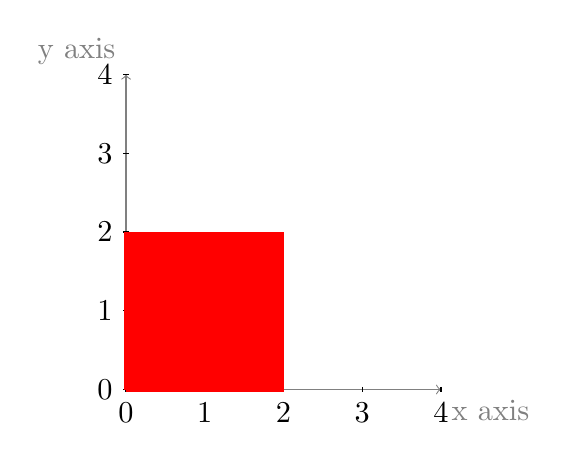
\begin{tikzpicture}
\draw[gray,->] (0,0)-- (4.0,0) node[anchor=north west] {x axis};
\draw[gray,->] (0,0)-- (0, 4.0) node[anchor=south east] {y axis};

\foreach \x in {0,1,2,3,4}
    \draw(\x cm, 1pt) -- (\x cm, -1pt) node[anchor=north] {$\x$};
\foreach \y in {0,1,2,3,4}
    \draw(1 pt,\y cm) -- (-1pt, \y cm) node[anchor=east] {$\y$};  

\draw[red, ultra thick] (0,0) -- (2,0);
\draw[red, ultra thick] (0,0) -- (0,2);
\fill[red] (0,0) rectangle(2,2);
\end{tikzpicture}
 
The formal definition for calculating the determinant of a 2 by 2 matrix is:
$$det(A) = (a*d)-(b*c)$$
where
$$A = 
\begin{bmatrix}
a & b  \\
c & d 
\end{bmatrix}
$$

For the matrix plotted above, the determinant is $(2*2)+(0*0)$. You can also see that 4.0 is the area, base (2) times height (2).

You can use the determinant to see what happens to a shape when it goes through a linear transformation. Let's scale the 2 by 2 matrix by 4:
$$
\begin{bmatrix}
8 & 0  \\
0 & 8 
\end{bmatrix}
$$
Plot it:

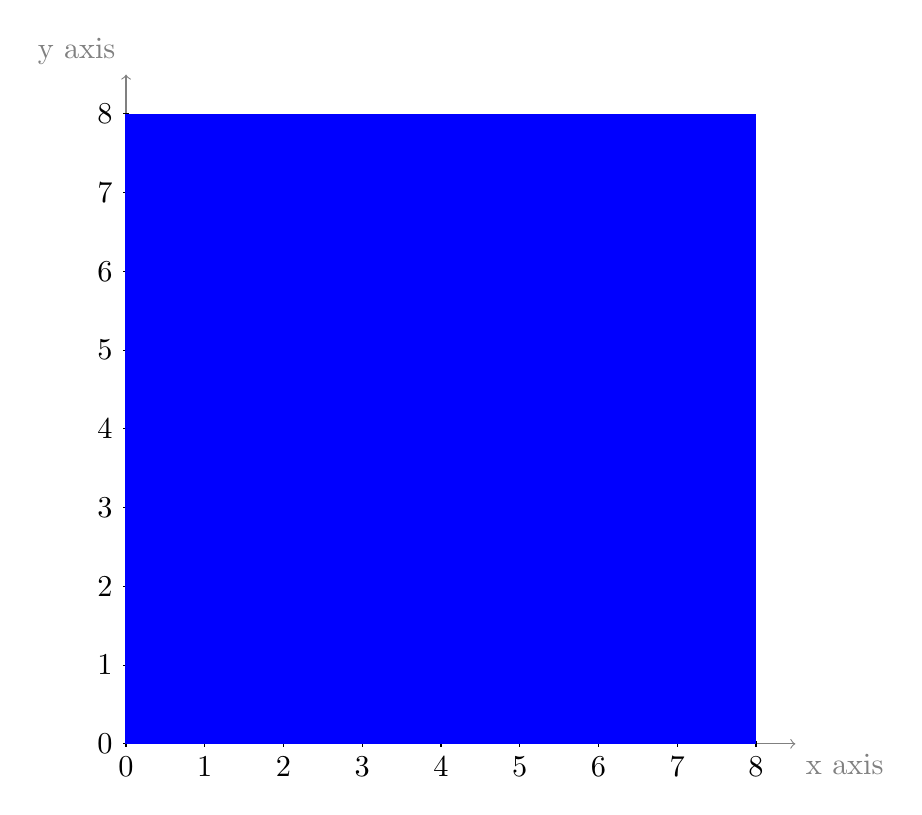
\begin{tikzpicture}
\draw[gray,->] (0,0)-- (8.5,0) node[anchor=north west] {x axis};
\draw[gray,->] (0,0)-- (0, 8.5) node[anchor=south east] {y axis};

\foreach \x in {0,1,2,3,4,5,6,7,8}
    \draw(\x cm, 1pt) -- (\x cm, -1pt) node[anchor=north] {$\x$};
\foreach \y in {0,1,2,3,4,5,6,7,8}
    \draw(1 pt,\y cm) -- (-1pt, \y cm) node[anchor=east] {$\y$};  

\draw[blue] (0,0) -- (8,0);
\draw[blue] (0,0) -- (0,8);
\fill[blue] (0,0) rectangle(8,8);


\end{tikzpicture}

Find the determinant. 

$$(8*8)+(0*0) = 64$$

You can see that scaling the matrix cubed the area.

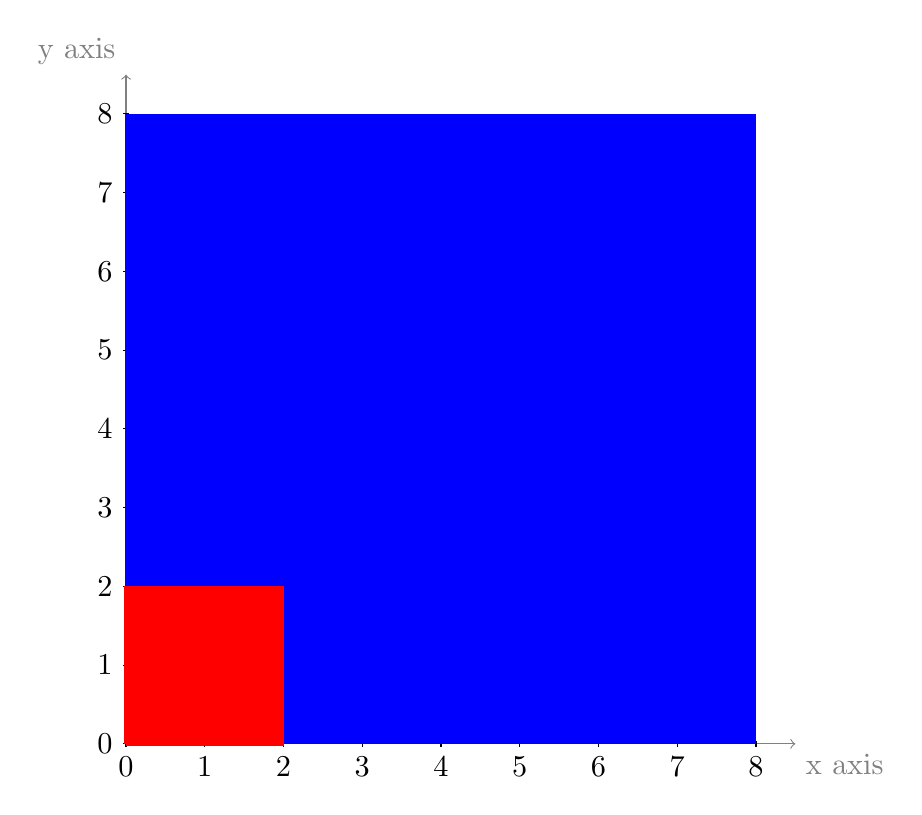
\begin{tikzpicture}
\draw[gray,->] (0,0)-- (8.5,0) node[anchor=north west] {x axis};
\draw[gray,->] (0,0)-- (0, 8.5) node[anchor=south east] {y axis};

\foreach \x in {0,1,2,3,4,5,6,7,8}
    \draw(\x cm, 1pt) -- (\x cm, -1pt) node[anchor=north] {$\x$};
\foreach \y in {0,1,2,3,4,5,6,7,8}
    \draw(1 pt,\y cm) -- (-1pt, \y cm) node[anchor=east] {$\y$};  

\draw[blue] (0,0) -- (8,0);
\draw[blue] (0,0) -- (0,8);
\fill[blue] (0,0) rectangle(8,8);

\draw[red, ultra thick] (0,0) -- (2,0);
\draw[red, ultra thick] (0,0) -- (0,2);
\fill[red] (0,0) rectangle(2,2);

\end{tikzpicture}
 
Let's plot this matrix
$$
\begin{bmatrix}
2 & 1  \\
4 & 2 
\end{bmatrix}
$$

\begin{tikzpicture}
\draw[gray,->] (0,0)-- (4.5,0) node[anchor=north west] {x axis};
\draw[gray,->] (0,0)-- (0, 4.5) node[anchor=south east] {y axis};

\foreach \x in {0,1,2,3,4}
    \draw(\x cm, 1pt) -- (\x cm, -1pt) node[anchor=north] {$\x$};
\foreach \y in {0,1,2,3,4}
    \draw(1 pt,\y cm) -- (-1pt, \y cm) node[anchor=east] {$\y$};  

\draw[red, ultra thick] (0,0) -- (4,2);
\draw[blue, ultra thick] (0,0) -- (2,1);

\end{tikzpicture}

One line overwrites the other. As you can see, the area is 0. The columns are linearly dependent.

Calculating the determinant for a 2 by 2 matrix is easy. For a larger matrix, finding the determinant is more complex and requires breaking down the matrix into smaller matrices until you reach the 2x2 form. The process is called expansion by minors. For our purposes, we simply want to first check to see if a matrix contains linearly independent rows and columns before using our Python code to solve. 

Modify your code so that is uses the $np.linalg.det()$ function. If the determinant is not zero, then you can call the $np.linalg.solve()$ function. Your code should look like this:
\begin{Verbatim}
if (np.linalg.det(D) != 0):
    j = np.linalg.solve(D,e)
    print(j)
else:
     print("Rows and columns are not independent.")
\end{Verbatim}

\section{Where to Learn More}
Watch this video on \emph {Linear Combinations and Vector Spans from Khan Academy}: \url{http://rb.gy/g1snk}

The Wolfram Demonstrations website has a fun, interactive demo where you can enter values for 2D and 3D matrices and see how the area or volume changes. 
\url{https://demonstrations.wolfram.com/DeterminantsSeenGeometrically/#more}

If you are curious about the \emph {Expansion of Minors}, see:
\url {https://mathworld.wolfram.com/DeterminantExpansionbyMinors.html}
\graphicspath{{../../Chapters/systems_matrices/en_US}}
\chapter{Matrices}
You've already had experience with matrices earlier in this module and also when you've used spreadsheets. In this chapter you'll learn the types of matrices and get an introduction to some of the special matrices used for various calculations. 

As you know, a matrix is a rectangular array of numbers arranged in rows and columns. The individual numbers in the matrix are called elements or entries. Matrices can be described by their dimensions. For example, a matrix with 2 rows and 3 columns is a 2 by 3 matrix.

$$\begin{bmatrix}
1 & 2 & 3\\
4 & 5 & 6 
\end{bmatrix}
$$

More generally, a matrix with $m$ rows and $n$ columns is referred to as an $m \times n$ matrix or simply an $m$-by-$n$ matrix, and $m$ and $n$ are its dimensions.

The general form of a $2 \times 3$ matrix $A$ is:
$$
A = \begin{bmatrix}
a_{1,1} & a_{1,2} & a_{1,3} \\
a_{2,1} & a_{2,2} & a_{2,3}
\end{bmatrix}
$$

\section{Types of Matrices}
Matrices can be described by their shape:
\begin{itemize}
	\item \textbf{Row Matrix:} has only one row.
	\item \textbf{Column Matrix:} has only one column.
	\item \textbf{Square Matrix:} has the same number of rows and columns.
	\item \textbf{Rectangular Matrix:} has an unequal number of rows and columns.
\end{itemize}

They can also be described by their unique numerical properties. Special matrices tht come in handy for certains types of computations. These are a few of the most common special matrices.
\begin{itemize}
	\item \textbf{Zero Matrix:} contains only entries that are zero.
	\item \textbf{Identity Matrix:} sometimes called the unit matrix, is a square matrix whose diagonal entries are 1 and all other entries are 0.
	\item \textbf{Symmetric Matrix:} a square matrix that equals its transpose.
	\item \textbf{Diagonal Matrix:} has nonzero elements on the main diagonal, but all other elements are zero
	\item \textbf{Triangular Matrix:} This is a special square matrix that can be upper triangular or lower triangular. If upper, the main diagonal and all entries above it are nonzero while the lower entries are all zero. If lower, the main diagonal and all the entries below it are nonzero while the upper entries are all zero. 
\end{itemize}

\subsection{Symmetric Matrices}
If you want to find out if a square matrix is symmetric, you need to transpose it. If the transpose is equal to the original matrix, then the matrix is symmetric.

To transpose a matrix, flip it over its diagonal so that the rows and columns are switched, like this:
$$
A = \begin{bmatrix}
a_{1,1} & a_{1,2} & a_{1,3} \\
a_{2,1} & a_{2,2} & a_{2,3} \\
a_{3,1} & a_{3,2} & a_{3,3}
\end{bmatrix}
$$
After transposing:
$$
A^T = \begin{bmatrix}
a_{1,1} & a_{2,1} & a_{3,1} \\
a_{1,2} & a_{2,2} & a_{3,2} \\
a_{1,3} & a_{2,3} & a_{3,3}
\end{bmatrix}
$$
Note that $A^T$ means the transpose of A. 

Let's see how this works for the following square matrix, A.
$$
A = \begin{bmatrix}
1 & 2 & 3 \\
2 & 4 & 5 \\
3 & 5 & 6
\end{bmatrix}
$$
Switch the rows and columns to get the transpose:
$$
A^T = \begin{bmatrix}
1 & 2 & 3 \\
2 & 4 & 5 \\
3 & 5 & 6
\end{bmatrix}
$$
Notice that $A = A^T$, so the matrix is symmetric.

What about matrix B? 
$$
B = \begin{bmatrix}
1 & 2 & 3 \\
2 & 4 & 5 \\
7 & 8 & 9
\end{bmatrix}
$$
Switch the rows and columns to get the transpose:
$$
B = \begin{bmatrix}
1 & 2 & 7 \\
2 & 4 & 8 \\
3 & 5 & 9
\end{bmatrix}
$$

Note that $B \neq B^T$. So B is not symmetrical.

\begin{Exercise}[title={Matrix Transposition}, label=matrix-transpose01]
Find the transpose of this matrix. Is it symmetric? 
$$A = \begin{bmatrix}
 		3 & -2 &4  \\
 		-2 & 6 &2 \\
 		4 & 2 & 3 
	  \end{bmatrix}$$
\end{Exercise}
\begin{Answer}[ref=matrix-transpose01]
$$A =  A^t = 
	  \begin{bmatrix}
 		3 & -2 & 4  \\
 		-2 & 6 & 2 \\
 		4 & 2 & 3 
	\end{bmatrix}$$
\end{Answer}

\subsection{Creating Matrices in Python}

Create a file called \filename{matrices\_creation.py} and enter this code:
\begin{Verbatim}
# import the python module that supports matrices
import numpy as np
# Use the function np.array to define a matrix that 
# contains specific values that you supply.
A = np.array([[ 5, 1, 3], 
              [ 1, -1, 8], 
              [ 6, 2, 1]])
# The transpose function returns 
A.transpose()
\end{Verbatim}
When you run it, you should see:
\begin{Verbatim}
array([[ 5, 1, 6], 
       [ 1, -1, 2], 
       [ 3, 8, 1]])
\end{Verbatim}
As you can see, $A\neq A^T$ so A is not symmetric.
Try another: 
\begin{Verbatim}
# create a matrix, B
B = np.array([[ 5, 1, 6], 
              [ 1, -1, 2], 
              [ 6, 2, 1]])
B.transpose()
\end{Verbatim}
When you run it, you should see:
\begin{Verbatim}
array([[ 5, 1, 6], 
       [ 1, -1, 2], 
       [ 6, 2, 1]])
\end{Verbatim}
B is symmetric. You can actually transpose any matrix using this function. But a matrix cannot be symmetric unless it is square. 

Try this code to see what happens when you transpose a rectangular matrix. 
\begin{Verbatim}
# create a matrix, J
J = np.array([[ 5, 1, 3, 0], 
              [ 1, -1, 8, 11], 
              [ 6, 2, 1,-7]])
J.transpose()
\end{Verbatim}
Note that transposing a rectangular matrix changes its dimension from 3 by 4 to 4 by 3. You should see a transposed matrix, but it's not symmetric.
\begin{Verbatim}
array([[ 5,  1,  6],
       [ 1, -1,  2],
       [ 3,  8,  1],
       [ 0, 11, -7]])
\end{Verbatim}

\subsection{Creating Special Matrices in Python}
 Use the same file to add this code for creating a zero matrix.
\begin{Verbatim}
# create an 8 by 10 Zero matrix.
 C = np.zeros((8, 10))
 C
\end{Verbatim}
When you run it, you should see:
\begin{Verbatim}
array([[0., 0., 0., 0., 0., 0., 0., 0., 0., 0.],
       [0., 0., 0., 0., 0., 0., 0., 0., 0., 0.],
       [0., 0., 0., 0., 0., 0., 0., 0., 0., 0.],
       [0., 0., 0., 0., 0., 0., 0., 0., 0., 0.],
       [0., 0., 0., 0., 0., 0., 0., 0., 0., 0.],
       [0., 0., 0., 0., 0., 0., 0., 0., 0., 0.],
       [0., 0., 0., 0., 0., 0., 0., 0., 0., 0.],
       [0., 0., 0., 0., 0., 0., 0., 0., 0., 0.]])
\end{Verbatim}
Add the following code to create an 8 by 8 Identity matrix.
\begin{Verbatim}
# create an 8 by 8 Identity matrix 
 D = np.eye(8)
 D
\end{Verbatim}
When you run it, you should see:
\begin{Verbatim}
array([[1., 0., 0., 0., 0., 0., 0., 0.],
       [0., 1., 0., 0., 0., 0., 0., 0.],
       [0., 0., 1., 0., 0., 0., 0., 0.],
       [0., 0., 0., 1., 0., 0., 0., 0.],
       [0., 0., 0., 0., 1., 0., 0., 0.],
       [0., 0., 0., 0., 0., 1., 0., 0.],
       [0., 0., 0., 0., 0., 0., 1., 0.],
       [0., 0., 0., 0., 0., 0., 0., 1.]])
\end{Verbatim}
As you progress in your studies you'll learn the importance of diagonal matrices and of extracting the diagonal of a matrix. Let's see how to extract a diagonal and then to create a diagonal matrix.
\begin{Verbatim}
# create a  matrix 
W = np.array([[1, 2, 3, 4], 
              [5, 6, 7, 8], 
              [-8, -7, -6, -5],
              [-4, -3, -2, -1]])
\end{Verbatim}
Extract the main diagonal using np.diag(<array>,<diagonal to extract>). 
Passing 0 as the second parameter specifies the main diagonal. A positive value extracts a diagonal from the upper part. A negative value extracts a diagonal from the lower part. Run this code then experiment passing other values to see what you get.
\begin{Verbatim}
print(np.diag(W,0))
\end{Verbatim}
When you run it you should see;
\begin{Verbatim}
array([ 1,  6, -6, -1])
\end{Verbatim}
You can also use np.diag() to create a diagonal matrix from a 1D array. In this case, do not pass a second paramenter.
\begin{Verbatim}
Q = np.array([1, 2, 3])
DiagArray = np.diag(Q))
print(DiagArray)
\end{Verbatim}
When you run it you should see;
\begin{Verbatim}
[[1 0 0]
 [0 2 0]
 [0 0 3]]
\end{Verbatim}
Python has functions for extracting upper and lower triangular matrices. Try these:
\begin{Verbatim}
print(np.triu(W))
print(np.tril(W))
\end{Verbatim}
You should see:
\begin{Verbatim}
[[ 1  2  3  4]
 [ 0  6  7  8]
 [ 0  0 -6 -5]
 [ 0  0  0 -1]]
 
[[ 1  0  0  0]
 [ 5  6  0  0]
 [-8 -7 -6  0]
 [-4 -3 -2 -1]]
\end{Verbatim}




%%%%%%%%%%%%%%%%%%%%%%%%%%%%%%%%%
%% Bookfooter.tex by Aaron Hillegass
%% Nov 8, 2020

\appendix

\chapter{Answers to Exercises}
\shipoutAnswer

\bibliography{references}

\printindex

\end{document}